\documentclass[10pt]{report}
\usepackage{graphicx}
\usepackage{graphics}
\usepackage{a4}
\usepackage{url}
\usepackage{fullpage}
\usepackage{moreverb}

% Report template authored V. Sorge, adapted S. Vickers.

\title{% This is the title of your document
{\normalsize Software Workshop Team Java (06-08165) 2010/11, Dr. E. Thompson}\\[2cm]
Project Report:\\
Space Runner Game}
\author{Team B3:\\
Daniel Cecil\\
Jere Ketonen\\
David Saunders\\
Michal Staniaszek
}

\begin{document}
\maketitle
\chapter*{Work Breakdown}
\label{work-breakdown}

\thispagestyle{empty}

% Obviously these need discussing and changing....
{\small

\noindent\begin{tabular}{|l||l|l|l|l|l|}\hline
  \textbf{Coding} & \textbf{Daniel} & \textbf{Jere} & \textbf{David}
 & \textbf{Michal} \\\hline\hline
 Datastructures & Contribution: 5\% & 10\% & 20\% & 65\%\\\hline
 \ldots & \ldots & \ldots & \ldots & \ldots \\\hline
\end{tabular}\vspace*{1cm}

\noindent\begin{tabular}{|l||l|l|l|l|l|}\hline
  \textbf{Report} & \textbf{Daniel} & \textbf{Jere} & \textbf{David}
 & \textbf{Michal}\\\hline\hline
 Introduction & Chapter~\ref{cha:introduction}: 100\% & 0\% & 0\% & 0\%\\\hline
 \ldots & \ldots & \ldots & \ldots & \ldots \\\hline
\end{tabular}

}     % This is the "}" that matches the "{" before "\small"

\tableofcontents
\thispagestyle{empty}

\begin{abstract}
  You should write a one-page abstract written as an ``Executive Summary''. It
  should be written for someone who is familiar with the Team Java module, so
  that there is no need for background or generalities. Rather, you should
  explain what is special about your project, and what you claim to have
  achieved. (One page maximum.)
\end{abstract}


\chapter{Introduction}
\label{cha:introduction}

This aim of this report is to give a overview of the team Java work we did for 11 weeks on a Space Shooter game and how it progressed from an idea on paper to a functional program.
It will be broken into sections covering important details on the design process, the way we worked and put the project together, the problems we faced, how we over came those problems and how we could improve the project futher with more time and resources.


Give a brief overview and guide the reader to the important points
in the remaining sections.

This template for your report also contains some examples of how to use some
{\LaTeX} elements and commands. In particular, there are examples for tables,
how to include figures, and various environments for bullet points or
enumerations.

For further information (and here is how to do a bullet list):
\begin{itemize}
\item look on the Team Java web page,\\
\url{http://www.cs.bham.ac.uk/internal/courses/team-java/current}\\
  (Click on ``Guidance''.)
\item google ``latex''
\item look at the \LaTeX book \cite{latex}
\end{itemize}


This is how to do numbered lists:
\begin{enumerate}
\item First point
\item Second point
\item \ldots
\end{enumerate}

This is how to do sections:

\section{Some topic}\label{some}

\section{Another topic}\label{another}

If you set a label with the \texttt{label} command, you can then use
the \texttt{ref} command to refer to that section -- e.g.
section~\ref{some}. This means you don't need to know about section
numbers. Note that \texttt{\~} means a space that cannot be broken
across lines.
 % needs doing...
\chapter{Requirements}
\label{cha:requirements}
\section{Functional User Requirements}
\label{sec: functional}

This section outlines the functional requirements which the system will be tested against. Functional requirements are what the system is expected to do and how to user interacts with the software. Each requirement is split into sub-requirements for ease of understanding and clarity.

\begin{enumerate}
\item \textbf{The human player is able to control one's spaceship}
\\* This is a core requirement needed to be able to play the game successfully in at least a single player mode without any crashes or bugs.
\begin{enumerate}
\item The user is able to use either a mouse or the keyboard's arrow keys to move the spaceship.
\item The user's spaceship is able to move freely along the x and y coordinates but not leave the frame's boundaries.
\item The user will be able to hold more than one key for diagonal movement where the movement speed much be normalised.
\item The user's spaceship will be able to be represented graphically on the screen.
\end{enumerate}

\item \textbf{The human player will be able to shoot}
\\* The aim of the game is to enable the user to destroy enemy ships and therefore shooting is a must-have requirement of the game.
\begin{enumerate}
\item The user will be able to shoot by tapping or holding the spacebar or the mouse button (left click).
\item The user's spaceship will have a type of weapon to use, this can be changed during the game (if implemented - dependant on future requirement).
\item The user's shot will follow a set path forwards (negative y-coordinate movement).
\item Shots which leave the frame's boundary will be removed from the game state.
\end{enumerate}

\item \textbf{Enemies will be created to be destroyed by the user}
\\* This is a core functional requirement that needs to be implemented to enable the user to progress through the game by shooting down opposing units.
\begin{enumerate}
\item Enemies will be spawned at set locations on the screen.
\item Enemy units are to have a set health limit.
\item Enemies will be able to be shot by any user spaceship.
\item Enemies are to be distinguishable from friendly user spaceships by using different shapes or graphics.
\item The enemy unit's health will be decreased when a user's shot collides with the enemy.
\item Enemy's will 'die' once all their health have been depleted.
\end{enumerate}

\item \textbf{Enemies are to be able to return a level of resistance}
\\* This requirement is needed to make the game more interesting by introducing the possibility of a player 'death'
\begin{enumerate}
\item Enemies are able to return shots towards the human players with the use of different weapons.
\item Enemies are able to move in certain paths (zig-zag, diagonal, straight, side-to-side).
\item If the player collides with an enemy the player will 'die'
\item 'Boss' enemies are to be introduced which fire more shots and have more health.
\end{enumerate}

\item \textbf{The game is to run continuously with set events occurring at regular intervals}
\\* This requirement ensures the game runs smoothly and that something will always happen. For example, to stop the incidence of no more enemies being spawned (so the game is playable).
\begin{enumerate}
\item The game is to implement a Timer class.
\item Enemies will always be spawned at set intervals during the game. These can be changed to be more or less frequent (if future requirement is implemented).
\item Each tick of the timer will move enemies, player units (depending on user input) and projectiles.
\item The game panel will be redrawn at every tick of the timer.
\end{enumerate}

\item \textbf{The game will be able to be multiplayer across the network}
\\* This requirement is necessary to fulfil the assessment criteria allowing for a second human user to play in co-operative mode with each other against the computer enemies.
\begin{enumerate}
\item Each human user will be able to select whether they will act as the host or the client PC.
\item Clients will be able to enter the Host's IP address to connect.
\item The host's game will start immediately after selection with clients dropping into the game at a set spawn point.
\item The game must be able to support at least two human players and a maximum of eight players (7 clients).
\item All users must be connected to the same LAN network.
\item All users must have similar game information on their screens (player, enemy and projectile positions).
\item With each tick of the timer (requirement 5) each player's screen will be updated with network data from the host.
\end{enumerate}

\item \textbf{The game must have a terminating clause}
\\* This requirement ensures that the game will end at some point.
\begin{enumerate}
\item Once a player's health has been depleted, that unit will 'die' and be removed from the game allowing other player's to carry on playing.
\item If a player collides with an enemy unit they will also 'die'
\item The player's score will be displayed on termination and if high enough will be recorded in a high scores table.
\end{enumerate}

\item \textbf{The game will include a Graphical User Interface (GUI)}
\\* This allows all users to be able to start the necessary game type as well as actually play the game with the information displayed on the screen.
\begin{enumerate}
\item The game will run from a single frame.
\item Panels are to be added to the frame: Menu, Game, Gameover.
\item The Menu Panel is to feature buttons corresponding to various game types and options.
\item The Menu Panel is to be accessible from within the game (Esc key).
\item The Game is to be able to be paused using the 'P' key.
\item The window is to be resizable allowing for full-screen play.
\item The Game Panel is to feature a scrolling 'star-like' background (black with white stars).
\item The game objects (players, enemies and projectiles) are to be represented by shapes or sprites (graphics).
\end{enumerate}

\end{enumerate}


\subsection{Attributes}
\label{sec: req_attributes}

\noindent\begin{tabular}{| l || p{6cm} | p{7cm} |}\hline
  \textbf{Attribute} & \textbf{Requirement No.} & \textbf{Comment}  \\\hline\hline
  Status & All & Approved - development started \\\hline
 Priority & 1, 2, 3, 4abc, 5, 6, 7, 8abch  - Mandatory. &  Mandatory requirements must be implemented.\\
 & 4d, 8defg - Important & \\\hline
 Effort & All & Deadline for code: 22/03/11 (10 weeks). Estimated 40 person-weeks for first release. \\\hline
 Risk & All & Medium probability of risk occurring. Large impact if assessment is not complete. High risk with networking code due to lack of experience. \\\hline
 Target Release & 1, 8a, 8h & v0.1 \\
 & 2 & v0.2 \\
 & 3b-f & v0.3 \\
 & 4, 5, 7 & v0.4 \\
 & 3a, 8b-g & v0.5 \\
 & 6 & v0.6 \\\hline
 Assigned To & All & 4 x Team Members. Requirements and tasks to be distributed at weekly meetings. \\\hline
\end{tabular}\vspace*{1cm}


\section{Non-functional User Requirements}
\label{sec: non-functional}

This section outlines the non-functional requirements. These requirements relate to the quality of the product and testing requires opinions and qualitative methods rather than quantitative feedback. The project has been split into different categories of requirement.

\paragraph{Usability} 
\begin{enumerate}
\setcounter{enumi}{8}
\item \textbf{To provide a simple, easy to use system in order to play the game}
\begin{enumerate}
\item A novice to the game should be able to gain understanding and play the game within 10 minutes of first playing.
\item Expert gamers should be able to grasp game concept within 1-2 minutes of playing.
\item The game should have a clean look and feel.
\item The user should feel in control of their spaceship with smooth movement and quick reactions.
\item The menu should have a standard, organised layout with minimal pages
\item The game should have a professional look
\end{enumerate}
\end{enumerate}
A user manual or help pages are not required due to the limitations on time for the assessment and the game itself is believed to be simple enough for most people to be able to understand.

\paragraph{Efficiency}
\begin{enumerate}
\setcounter{enumi}{9}
\item \textbf{The game should be constantly quick to respond}
\begin{enumerate}
\item The game should run at a constant quick speed without any lag.
\item The user's input should have an almost instant effect on the game.
\item Network play should be stable for 95\% of the time.
\end{enumerate}
\end{enumerate}

\paragraph{Dependability}
\begin{enumerate}
\setcounter{enumi}{10}
\item The game should run first time, all of the time as single player or host.
\item Network clients should be able to drop-into the host's game within 5 seconds.
\end{enumerate}

\paragraph{Environmental}
\begin{enumerate}
\setcounter{enumi}{12}
\item The game should run on the platforms detailed in the below section (system requirements).
\end{enumerate}

\paragraph{Development}
\begin{enumerate}
\setcounter{enumi}{13}
\item The project should be developed using appropriate software engineering practises within the time frame for the assessment.
\item The project must be written in the Java programming language.
\end{enumerate}

\paragraph{Operational}
\begin{enumerate}
\setcounter{enumi}{15}
\item The multiplayer game must be able to run on any LAN with the IP addresses given.
\item High scores will remain stored in each copy of the game until they are overridden by a higher score.
\end{enumerate}

\section{System Requirements}
\label {sec: system_requirements}
This section details the requirements and physical devices needed to play the game successfully.

\begin{enumerate}
	\item The game is to be written in the Java programming language.
	\item All user PCs will need to follow the system requirements for Java 6
	\begin{enumerate}
	\item Windows 7, Vista, XP, 2000, Server 2008, Server 2003. All 32 and 64-bit operating systems
	\item Mac OS X
	\item Most Linux distributions
	\item Solaris
	\end{enumerate}
\item Keyboard and Mouse are required (with Western layout)
\item For multiplayer, all users will need to be connected to a local area network (LAN) at least
\item Monitor and graphics card with at least a resolution of 800 x 600 
\end{enumerate}

\section{Future Requirements}
\label{sec: future_requirements}
Requirements 1 to 17 are aimed at the first release which is as far as the project is aimed to go. However if the project is ahead of schedule the progress will be re-evaluated and requirements from this list will be introduced depending on complexity and remaining time and resources available.
\begin{itemize}
\item Power Ups
	\begin{itemize}
	\item Increased health
	\item Increased shot damage
	\item Enemies freeze
	\item Move quicker
	\end{itemize}
\item Boss Fights
	\begin{itemize}
	\item Enemy unit with lots of health - harder to kill
	\item Enemy has greater weapons
	\item Enemy does not move off screen (has to be killed)
	\end{itemize}
\item Different Weapons
	\begin{itemize}
	\item Greater damage
	\item Single-shot
	\item Multiple direction shooting
	\end{itemize}
\item Increasing Difficulty
	\begin{itemize}
	\item Enemies spawn more often in larger numbers
	\item Enemies have greater damage
	\item Enemies have greater health
	\item Enemies shoot more often
	\item More boss fights
	\end{itemize}
\item Background music added
\item Endless mode (player respawns)
\end{itemize}
\chapter{Design}
\label{cha:design}

This section is crucial. Describe the overall structure of your
program at a suitably high level of abstraction. For instance, UML
diagrams or informal box-and-arrow diagrams can be used to describe
program structure. Be sure to describe the MVC structure used. Note
that code listings or screenshots are not appropriate here. An
important point is how you have divided the project into modules
that different team members can work on, and how these are then
integrated. For example, you could use interfaces to describe a
clean boundary between modules, so that some team members use the
functionality provided by the interface, while another team member
implements it. Bear in mind Software Engineering principles of good
design like coherence and coupling.

\section{Release Plan}
\label{sec: release_plan}
This section outlines the proposed release plan of the project. It has been decided that the project will take the incremental approach of software development with acceptance testing taking place at each stage. The six internal releases will be implemented consecutively to bring the project to the first public release within the 10 week timeframe.

\begin{itemize}
\item \textbf{Version 0.1:} Basic player spaceship (Java shape) on screen with controls and movement.
\item \textbf{Version 0.2:} Basic shooting from the player's spaceship.
\item \textbf{Version 0.3:} Static enemies on the screen, player able to shoot the enemy and score incremented.
\item \textbf{Version 0.4:} Enemies have movement with the use of paths, are able to shoot back and collide with players.
\item \textbf{Version 0.5:} Background scrolling, enemies are spawned at regular intervals at set points using a timer.
\item \textbf{Version 0.6:} Multiplayer networking implemented.
\end{itemize} This brings the project to the first public stable release which satisfies the requirements for the assessment. It time is available certain future requirements (section \ref{sec: future_requirements}) towards the second public release.

\section{Class Design}
\label{sec: class_design}
Below shows a diagram of how the project is to be organised in terms of classes and packages (dotted lines show packages).
\begin{figure}
 \centering
 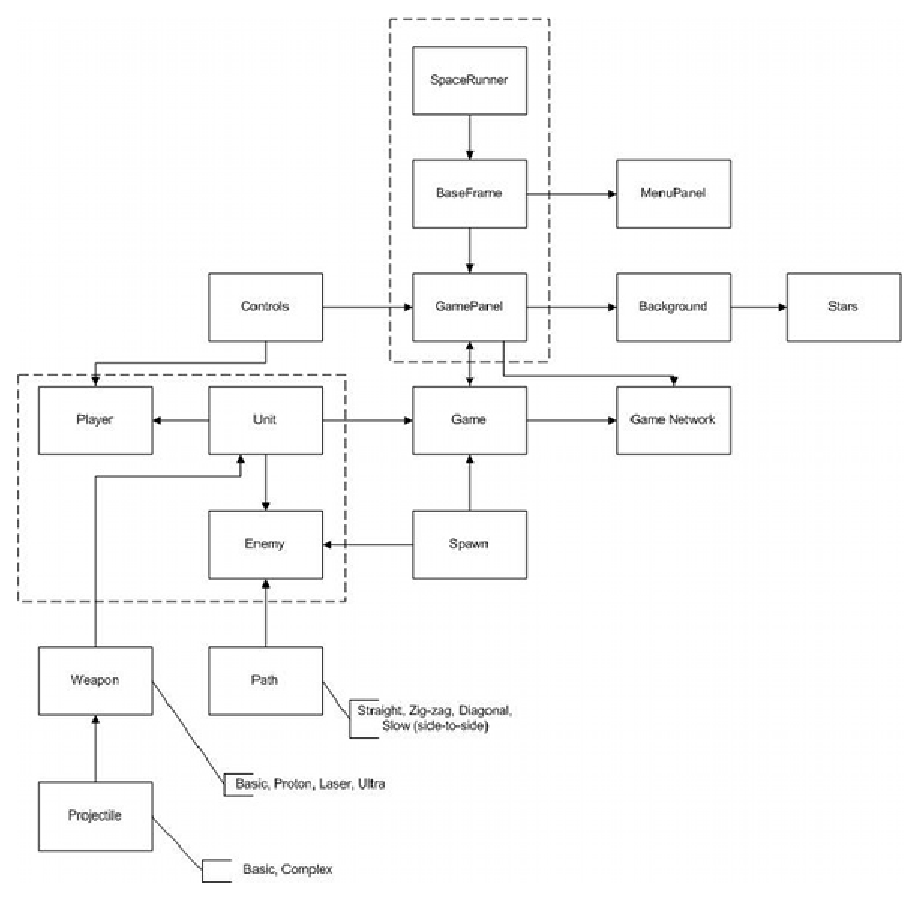
\includegraphics{class_diagram_small.eps}
 \caption{Proposed class diagram for the project}
 \label{fig: class_diagram}
\end{figure}

\section{Implementation}
\subsection{GUI and Controls}
The GUI was written using the standard JFrame and JPanel layout. A menu and a game panel were embedded inside the JFrame using a panel with a CardLayout. The menu and panel are part of the card layout, and can therefore be switched to very easily by referring to the name given to the CardLayout when each panel is added. There were some problems implementing a switching method to switch out the game and menu when either was required. Since the GamePanel is controlled by a timer, it is not possible to throw exceptions out. Therefore, another method was devised, by which the frame would call a method in the currently active panel to check if a `switch' flag was set. Based on this flag, the frame would change the panel that was currently being displayed, along with performing relevant actions. For example, when the menu is accessed while playing the game, the game has to be paused, and so the frame accesses a variable in the GamePanel which controls whether the game logic is progressing or not.
\subsection{Menu}
The menu is composed of simple objects such as rectangles that switch out using card panels. These card panels allow for easy switching of panels when an action is performed such as for our game when the user clicks to start a single player game. The way the panel detects what the user wants us by using mouse listners and checking if the mouse is within the bounds of the rectangle when the mouse button is clicked. Once clicked the panel will switch out to the coresponding panel action that was designated as the action of the "on click" of the rectangle. Another thing to note is that when escape is pressed suring game play the game will pause and switch the panel out back to the menu where the user can then either start a new game or resume the current game.
\subsection{Controls}
The controls for the game were implemented by using mouse and key listeners as to allow the user the choice of input method. The main way the controls work is by first detecting if the keyboard or mouse is being used and then using the apropriate method. For the mouse it would get the current pointer location and move the ship to that location on screen as well as listening for mouse button presses to triger the shooting method. The keyboard worked by detecting which key was being pressed and setting a boolian value to be true, this allowed the user to press multiple keys at once to move the ship diagonaly while also shooting. The control class was embeded into the game panel class so it ran when ever the game was started. Using the boolian values from the control class then decided upon where the ship would move to and if it was shooting or not.
\subsection{Game Logic}
The game logic is run in a loop that is controled by the game timer. The timer decideds on the frame rate of the game which affects the speed of which objects such as projectiles can move. Also within the game logic loop major components to the game such as collision detection and array pruning are called from the logic method. This part of the came could be said to be the game core that calls all the neccesary methods.
\subsubsection{Overview}
The game logic was written as a part of the program that could be used easily without any knowledge of the actual processing going on inside. The game logic is made up of a series of arrays, each consisting of objects that are part of the game; spawns, players, enemies and projectiles. These arrays are modified by the game in order to update the current state of the game. The arrays can be accessed by any class via getter methods, and objects can be added and removed if necessary. The logic can also perform removal of objects on command using certain pruning methods which are described later. The game logic also has methods to move all objects on the screen to new positions. The objects inside the arrays are manipulated inside the game panel using the methods of the game class. After logic has been done on the arrays, the panel then draws the objects inside the arrays.
\subsubsection{Collision detection}
The collision detection is na\"{i}ve, and done in two separate stages. Collisions of enemies with player projectiles is done first, and then collisions of enemy projectiles with the player, and enemies themselves with the player. This method is quick, and is not particularly computationally intensive given the type of game that we have written. Whether a collision actually occurs or not is defined by using a rectangular `hitbox' which surrounds the unit or projectile. If the hitboxes overlap, then the damage that the bullet carries is transmitted to the unit, and if the unit's health drops to zero or below as a result, the unit is removed from the array. The projectiles is removed from the array when it collides with a player or enemy object. Doing this gives quite a realistic feeling---it is not usual that a projectile passes through an object. However, implementing weapons that travel through units would not be problematic either, given the structure of the code. In order to avoid concurrent modification problems, enemies and projectiles that must be removed from arrays must first be stored in a secondary arraylist, which is then used to remove objects from the original array once all of the collisions have been checked.
\subsubsection{Array Pruning}
So as not to overload the memory of the computer with a huge number of objects, the arrays in the game are pruned of projectiles and enemies that are no longer within the visible area of the screen. This is done by creating a rectangle the size of the frame window, with the same coordinate space, and then, avoiding concurrent modification, removing the objects whose locations are not within the bounds of the frame rectangle. This also means that less processing is necessary during collision detection, and there are fewer objects that must be dealt with.
\subsection{Game Entities}
\subsubsection{Units}
For the units, we defined an abstract class that would contain all methods that would be necessary to access the basic information about the unit such as health. The game contains two subclasses of the unit class, player and enemy. In each of these classes, there are some parts that are specific to the requirements of those objects. For example, enemies have a method to get the value in points for destroying them, and the player class has a method to increment the score for that player. Using an abstract class meant that the subclasses already had all the necessary methods for access, and only needed some simple additional methods that were specific to the type of unit, and this saved writing quite a lot of unnecessary code. Each enemy unit moves based upon a path. Paths consist of a single equation, along with some directional variables to determine the next position of a unit based on its current position. Each time the game logic is run, this method is called with the object's current location, and returns the location that the object is due to move to next. This sort of implementation of paths allows for a robust method of control for both enemies and projectiles, and can be used to create a variety of interesting path types relatively easily, which allows for good extensibility. These paths also mean that the speed of units and projectiles can be controlled by using some sort of speed variable to increase the multiplier on the default additions to the coordinates, which would be very useful if there were to be difficulty levels added.
\subsubsection{Weapons and Projectiles}
The weapon and projectile classes are fundamental to the gameplay of the game. The weapon class is an abstract class which is intended to allow for quick addition of new weapon types into the game. Each weapon has a fire method which causes the weapon to create a new arraylist containing a number of projectiles specified by the method. This means that it is simple to add new projectiles to the game logic from quite a high position based on object orientation. Once one has a reference to a unit, it is only necessary to get the reference of the weapon, and then add the return array of the fire method to the game logic when one wants to cause weapons to fire. Each weapon has a fire rate, which is used by the logic to determine whether the weapon's fire method should be called or not. This allows for precise control of the weapons firing.

Projectiles are very simple objects which move based on paths. Each projectile object contains some data about which player it was spawned from (if it was), and details about its damage.
\subsubsection{Spawns}
The Spawn class is used to create new enemies during the game. The game has seven different set spawn points at regular intervals along the top of the screen, these points are held inside an array within the Spawn class. The class is currently able to spawn three types of enemy units: default unit which is abstract so that future types of unit can be created, boss enemy which is harder to shoot as it has increased health and different weapons as well as moving along a different path and finally the basic enemy unit which makes up the majority of the game. The spawn methods are called on the Spawn object in the GamePanel class at regular intervals in the game cycle (timer). There are various different types of spawn options available:
\begin{itemize}
	\item Spawn 1 unit at a given point (0.8\% chance of it being a boss enemy).
	\item Spawn a given number of units at the same given point.
	\item Spawn a given number of units at the same random point.
	\item Spawn a given number of units at different (chance of it being the same) random point.
\end{itemize}
Each of these methods returns an ArrayList of Units which can then be drawn in the render method in the GamePanel class. The Spawn class is abstract and can be modified in the future to add new types of enemy, the frequency can be changed in the GamePanel of how often units are spawned too.
\subsection{Network}
Networking is based on a client-server principle. Upon choosing the multiplayer option in the menu, the player is given a choice of hosting or joining a game. Depending on the option chosen, the game panel is initialised with server or client object which perform different tasks. When a client connects to the server via an input IP address, the server receives a reference to the client, which it then stores in a map. This map is used to get references to clients when data has to be sent to them. With a map, it is easy to send either to all clients, or choose a specific client to send data to. Client connections are dealt with by a handler, which sits in its own thread and waits for connection attempts to the server. When a connection is received, the handler adds the connection to the server's map via the interface, and the client immediately begins receiving any data from the server. Each individual client is embedded inside a class which contains methods to perform specific actions such as sending data over the network. The client and server perform interactions by first sending a string containing some information about the message that is to be sent next, and then sending the message. This method of communication is facilitated by a listener which runs in its own thread and constantly listens for commands coming in. If a command is received, a method in the socket is called to execute the request. This well structured communication method means that all communication can be handled in the correct way for that particular command. The method by which data is communicated over the network is via game state objects, which contain all the data needed by the game to run correctly; all the arrays, and boolean variables representing whether the game is running or not, along with a few others. The game state is capable of doing some processing, in order to reduce the data that is transferred over the network. A client first receives data from the server, and then runs its logic on it, moving projectiles fired by all units, and moving the player location. Each loop, the current state of the game is made into a new game state. This game state is then compared against the game state that was received from the server at the start of the loop. All objects that are the same in both game states are ignored---only new objects and the player reference are passed to the server, which reduces load on the network and also makes it easier for the server to collate the data into a single new game state which combines data from all clients which are currently connected. The server takes the new amalgamated game state, performs logic on it, and then sends it out to all clients, and the cycle continues. This method, along with the client storage method means that clients can drop in and out of the game without any wait time. In order to facilitate the transfer of objects over the network, upon object creation, each object is given a reference which will allow checking of the objects even if they are duplicated later, which is necessary for the removal of old objects.
\subsection{Graphics}
Graphics is implemented using a map stored in the game panel class. This map is initialised upon loading of the game with images from the relevant locations. Each object which must be drawn has an image reference string, which refers to the string that the image was added to the map with. When the object is drawn, the image reference is used to retrieve the image for that particular object, which is passed to the draw method of the object, which then draws it. Using this method meant that it was not necessary to pass images over the network, which would greatly slow communication due to the relatively large size of images. However, this method could, in theory, lead to the modification of the image files which are used to draw objects. In actuality, this will have no real effect on gameplay, since the size of the images are not at all considered when processing game logic.
\section{GUI Design}
\label{sec: gui_design}
The GUI will be fairly simple and initially the on-screen components will be made up of shapes (Java objects). The initial sketches are shown below which were created in the first week of development to aim understanding of the project.\\
\begin{center}
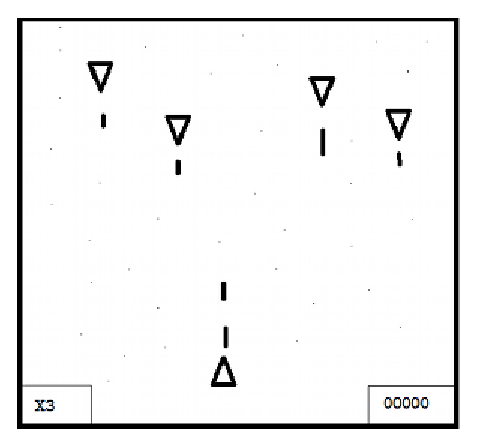
\includegraphics{GUI1.eps}

\includegraphics{GUI2.eps}
\end{center}
The menu screen (right) will have buttons that allow the user to select different types of game play, for example single or multi-player, as well as being able to exit the game or select different options. The menu is also accessible from within the game using the Esc key.\\\\
The game is to be implemented in a single window (frame) with different panels added (i.e. menu and game panels). The frame is to be resizable (including the layouts of ships) to allow the user to change the game from the default size.\\\\
In the Game Panel (left) the objects are represented as shapes. These are to be replaced with sprites (images) if the project allows sufficient time.
%%% Local Variables: 
%%% mode: latex
%%% TeX-master: "report"
%%% End:  % Dan to finish
\section{Testing}
During our initial discussions, we made some simple plans for how we would attempt to test each part of our program. Since each member of the team would be writing some parts of the code, it seemed to make sense that whoever wrote the code should test it as well. We decided that it would be a good idea to use JUnit tests, since these allowed for the mass testing of all classes in the program once everything was written. If we were to use another testing method, it would likely result in having to run some part of the program and check that its output was correct, or use a multitude of print statements to check that the program was running correctly, which would lead to having to trawl through a significant amount of data and pick out relevant parts, which would likely be very difficult to find, given that bugs do not necessarily occur frequently, and when they do, the signs are not obvious when looking at output. Once we had actually started the project, however, it became obvious that many parts of the game were not conducive to testing. For example, testing controls with JUnit is possible, but not particularly easy. The easiest way of testing the controls is simply to play the game, see if there are any problems, and then attempt to fix them. As development progressed, we discovered that writing tests before or after writing code meant that our development speed slowed significantly. We would spend quite a while writing tests to make sure that relatively simple parts of the code worked correctly, when it was obvious from playing the game that everything was as expected. Eventually, we decided that using JUnit was slowing us down too much, and did not actually provide as much benefit as we had initially hoped that it would provide, and we each used testing methods that we usually used when programming. Mostly, this involved reading the output at specific parts of the program that we knew would contain problems. Of course, testing was only done if something didn't work properly---there was no need to test something that didn't seem to be broken. Since we were running the game regularly and playing it to check if the code we had written was doing what it was supposed to, we believe that any bugs we had were spotted far more quickly this way than by laboriously writing JUnit tests and then using them to check that everything was working properly. By playing the game, we could test all the conditions that we would expect the code to work in, and if anything was broken, we would move to the output reading method, which in most cases worked without a problem. Printing out variables or arrays to see their current state allowed us to quickly see where the problem lay. There were a few times where this method did not allow us to solve the problem, and in these cases we went to the built in debug tool in netbeans. By stepping through each part of the program, or parts of the program that we thought were causing the d problem we could see the state of all variables in an organised way, and to step into methods that were part of the execution process, to check if there was some kind of error we were making in the order that code was executed.

We think that the main problem with the lack of success of the JUnit tests was the fact that the code distribution between members was not particularly even. As such, some members perhaps didn't understand the workings of a certain part of the program enough to write a test for it, and so tests were left unwritten. Since towards the end of development, there were only really two of us working on the code, we did not have sufficient time to test the entire code base, as we had to concentrate on writing the parts of the code that were required to complete the program. Perhaps if we had split the work in a more appropriate way, to allow everyone to work on some part, rather than ending up with two of us working on everything, we would have had enough time to write proper tests for everything. Another way that we could have solved this problem would have been to have one member who was responsible for testing all of the code, and not write any actual game code themselves. However, this person's understanding of code would have had to have been better than that of those writing the code, in order to be able to test everything correctly. Given the skill levels of members in our team, it is unlikely that this would have been possible, as the majority of the code would probably have not been written, since the person with the best understanding of code would probably be the one who would be needed to write most of the complex code, and other team members would likely be unable to test the code that that person would have written. Overall, however, apart from the networking code, we believe that everything has been tested to a relatively satisfactory standard by using only the testing methods that we have used. No major bugs in the code have been discovered yet, and as far as we are aware, the minor bugs have no real impact on gameplay.
\section{Validation} % Michal

\chapter{Project Management}
\label{cha:management}

\section{Development Methods}
\label{sec: development_methods}

We discussed the possible use of software engineering techniques we could utilise to make things easier and to ensure success and good planning. In a way it was hard, since we have no concrete experience about how much work a single software engineer can do and so forth.

\subsection{Weekly Meetings}
In the weekly meetings we discussed our progress so far on the whole project and any problems that had arisen on the week and how we could get around them and fix them. We went over our plans of what we would have to have done during the next week and revised if it still was a good idea and possible to implement at that stage. After deciding what we wanted to accomplish in the next week we tried to split the tasks evenly amongst us.
\\ \\
We usually had two meetings a week, one on Tuesday and one on Thursday with the demonstrator. After we got feedback from the demonstrator we reviewed our plans. Depending on what we discussed we usually wrote logs and drew some rough drafts about what to do. Our main communication medium has been Facebook. We formed a group there where we only have the members of our team and we have been dealing with assigning tasks over it and talking over any problems we might have. I have been quite surprised how well it has worked for a thing like this.

\subsection{Incremental Stages}
We decided to build the base game first, without anything fancy in it, as in the absolute core of the game. So we started out making the ships with just shapes and not sprites. After we got that to render properly, we started adding movement, opponents, spawning and shooting. \\\\
Basically we built the game in incremental stages, first making the core and then adding functionality on top of that. The goal was to have a working copy with more functionality at the end of every week, according to our schedule and plans. I think we managed that fairly well. At the very start we decided to try to keep the game at a bare minimum, no extra fancy stuff added or even planned very far until the core was working well, since we knew the hazards of getting stuck with planning and daydreaming without getting anything worthwhile working in the end.

\section{Planning}
\label{sec: planning}
We ended up with the idea of trying to document everything as well as we can and use weekly meetings to plan out the tasks for that week and where we want to be after it. So we set our iteration period to last a week and assigned tasks at the start of it. Requirements documentation and user requirements was among the things we knew are critical if you want a project to succeed in the timeline it has been given.\\\\
Trying our best to decide how much time to use on each part and how to divide the tasks in even portions, so that the contribution would be spread evenly amongst us. But as said above, we found it to be rather difficult since we had no clear concept of how hard it would be to code networking and other parts we had no experience about.\\\\
One thing that was a bit daunting was the team work itself, since no-one of us had any experience in it either, so how would it work if we had to work on a class that someone else was working on already and how to arrange it all so that it would not get too messy.
In the end we drew a rough diagram on how to organise our packages and classes and a basic timeline of when we would want each version to be out and what would it entail.

\section{Testing}
\label{sec: se_testing}
Testing is obviously and important part of any software development. At the very start of the project we decided to test everything well and throughly, if possible. We didn't have any experience with JUnit or testing in general, apart from the things we have done to debug our code and show testing with main methods during the first year.\\\\
After the lecture on testing and some help with the demonstrator we set up our tests and managed to test everything we had done so far and it all seemed to be in order. At the next stages of the project, I must admit, that we did not really utilise JUnit testing until the very end. But this does not mean we did not test everything. Everyone took care that the code they committed was tested with main methods and different kind of System.out.print commands.
 % Jere

\chapter{Conclusions}
\label{chap:conclusions}


Evaluate what you have achieved in your project in objective terms
(not just things like ``we are all happy with the result''). What
are the strenths and limitations of your project? If you had more
time, what could you add? If you could do it all over again, what
would you do differently? Are there general things about software or
team management that you have learnt in this project that you could
apply if you were going to work on a (perhaps completely different)
team project in the future?


\appendix
\section{Facebook Group Discussions}
\begin{verbatim}
Dan Cecil This is what I suggest we do over the weekend.... feel free
to comment or change anything:

Dan Cecil: finish requirements and design

Michal Staniaszek: validation/testing?

Jere Ketonen: Software Engineering practises (talk about weekly
meetings, incremental stages, tasks and revisions etc)

David Saunders: Team weekly log / introduction to the project?  on
Friday Jere Ketonen How much do we have to write about the stuff?
Sunday at 18
 
Dan Cecil Not sure really, I'm just going on however long it
takes... suppose a couple of pages maybe? :/

It's due in for 10am on Friday and needs to be bound etc so I suggest
we try to finish it for Thursday afternoon?  Sunday at 21

Jere Ketonen www.shaedar.com/finalreportse.rtf <-- This is what I have
so far. What should I add/edit?  Monday at 13

Michal Staniaszek I have no suggestions to make as I have no clue
about software engineering...but if possible, make it longer
somehow. Also, what is validation in this context?  Monday at 21

Dan Cecil Hi Jere, yer that's probably enough talking - maybe go into
a bit more detail if you can find something to talk about... do you
think we need Gantt / activity-on-arrow charts?  Yesterday at 04

Jere Ketonen Well.. everything is probably a plus, but I dont know. It
might be a bit overkill, or not. I mean some of the stuff we'd
probably just have to improvise from our heads since its kind of silly
to draw those after the project, I think.  Yesterday at 08



Dan Cecil Morning guys!  All good work so far....  I don't mind
putting the report together and filling in the gaps etc. If you could
try to get it to me (or SVN) by Wednesday afternoon and I'll finish it
on Thursday and hopefully get it bound and submitted in the afternoon
(it's due 10am Friday so would rather get it in on Thursday).

We also need to decide and agree on the work breakdown for both the
coding and the report... should be fairly straight forward (fingers
crossed).

Thanks, Dan on Monday

Michal Staniaszek I've submitted the testing part of validation and
testing to svn.  on Monday Dan Cecil All good!

For the testing part all you really need to do is go through the
requirements (user functional and non-functional) and compare them
against our game.

You can mention that we used JUnit to test the integrity of the code
but try to do...See more Yesterday at 04



Michal Staniaszek Please commit any progress made on the report to
svn.  on Sunday

Michal Staniaszek We need to decide who writes each part of the
report. Everyone should probably contribute to the section which
details why we coded things in the way we did, because we all wrote
code. As for the other parts, the software engineering part is left to
those of you who know what you're talking about. If anyone has a list
of the sections that need to be covered, please post it.  last
Thursday Dan Cecil Ok, I'm working on the Requirements (spec) and
Design.

The should be a LaTex template on SVN which shows the stages,
basically: 25 March at 02

Dan Cecil ‎- Introduction - Requirements - Design - Testing - Project
Management ...See more 25 March at 02

David Saunders Dan, we are going to have to have an section talking
about what the code does as well, breaking it down and explaining its
workings.  25 March at 12

Dan Cecil Do we really need that though? There's nothing in the slides
about doing so and I think that's the purpose of the
demonstration. The report is more to do with the process involved and
how we managed it etc. Suppose you could reference parts ...See more
25 March at 14



Jere Ketonen Tell me how it went when you know :X last Thursday Dan
Cecil Will do :) I take it you've told Errol etc that you won't be
there?  24 March at 14



Dan Cecil Good work guys! Are we going to meet up before the
demonstration tomorrow so we can decide who's doing what at the
presentation?  I say about 12 in the common room?  about a week ago
Michal Staniaszek I'll be there around 1 or so.  23 March at 18

Dan Cecil Ok cool, does anyone else find it hard to stay alive for
long or is it just me? Too many enemies firing but good work and no
real need to change it.  23 March at 19

Jere Ketonen I like the chaos atleast :D 23 March at 20 · 1 person
David Saunders I will be in for midday to check over stuff and do last
min tweaks.  24 March at 11

Dan Cecil I'll be in around 1 ish 24 March at 13


Michal Staniaszek I'm done with the networking. You can see actions of
the server on the client and the client on the server. It's super
jerky and a lot of the projectiles are lost, but I don't have the time
or willpower to fix it.  about a week ago

David Saunders Small bug, if the game is left open for 5 or so min the
game starts to lag (have to be playing the game not on the menu.
Could be a problem with pruning arrays maybe?  will look into it once
I've done the menu about a week ago Michal Staniaszek Yeah, I noticed
this as well. Not sure what's going on.  22 March at 18

David Saunders Hows the music btw? should I change it for something
else or is it fine?  22 March at 18

David Saunders Only noticed because I was checking if it looped or not
22 March at 18

Michal Staniaszek No idea, can't hear any music.  22 March at 18

David Saunders should be a mid file playing in the frame.  22 March at
18

Michal Staniaszek Yeah, I noticed.  22 March at 18

David Saunders replace the sequence line with this and try again, can
then know if its down to file location or not Sequence sequence =
MidiSystem.getSequence(new
URL("http://tinpan.fortunecity.com/hiphop/6/pop/e/Europe-FinalCountdown.mid"));
22 March at 18

Michal Staniaszek Doesn't seem to work either.  22 March at 18

David Saunders interesting...is working fine here with both.  22 March
at 18

Michal Staniaszek Awell. As long as it works in the jar, it should be
fine.  22 March at 19

Michal Staniaszek With regards to the bug, it doesn't seem to be a
problem with projectiles, as I can see that the server isn't sending a
massive number of them. Also, could you get the frame multiplayer
working asap, because it's rather a bitch to test client and server
interaction at the moment.  22 March at 19

David Saunders I have to intergrate what Jere did so will take abit of
time making some more methods and finding out which parameters are
needed since hes basically covered the GUI side of the menu while I
have covered all the switching out so far.  made it...See more 22
March at 19



Jere Ketonen I've basically just created a fancier looking panel for
the mainmenu, but I still have to implement changing the panels and
all that stuff and I've got no idea how to do it, so I wont upload it
until I get it done, if I even manage.  about a week ago David
Saunders the panel changing stuff is in mine, so if you want you can
use that as the framework for the menu? as all the panel changing is
currently done in the frame.  22 March at 17

David Saunders All ive done is just use the buttons to change some
fields which affect some stuff in the frame for the switch 22 March at
17

Jere Ketonen Uploaded the menu class Ive made, incase you want to try
to get it to work somehow aswell. Looks a bit fancier than the normal
button stuff, but dunno.  22 March at 17



David Saunders Jere Ketonen continued

about a week ago

David Saunders Jere Ketonen how to make a branch

about a week ago

Jere Ketonen Well I've been working on the mainmenu aswell, like David
but my code is totally different, so how can I branch it out or
whatever?  about a week ago Michal Staniaszek svn copy trunk
branch/[branchname].  22 March at 16



Michal Staniaszek Networking is semi-working. Projectiles from clients
are bugged, and you can't see the player, but the client gets data
from the server no problem.  about a week ago

David Saunders Jere Ketonen Just want to know if you are going to be
at the demonstration on Thursday or not since its the final
demonstration of our game.  about a week ago Jere Ketonen No, I wont
make that, there werent any cheap enough flights available around that
time :< 21 March at 16



Michal Staniaszek I believe that I have got stuff being sent over the
network.  about a week ago

Michal Staniaszek Right, I've changed the way that the images are
dealt with. The commit for revision 175 details a little
more. Basically, there's a map of BufferedImages in the game panel,
and when something wants to draw, it uses that map to find how it
should draw the object.  about a week ago

Michal Staniaszek Jere Ketonen, David Saunders. Please do some work on
the parts that I suggested below. We need to have this finished by
Thursday, preferably Wednesday. I don't particularly want to have to
mess around with stuff an hour before when we're supposed to
demonstrate.  about a week ago Dan Cecil I've just fixed the
controls.... something less to worry about.  20 March at 15

David Saunders ‎Dan Cecil you caused another bug doing that as you can
now move outside the window.  Michal Staniaszek - Main problem is that
I have no idea really how to link the two together...I uploaded a
start but I don't even know if im going in the ri...See more 20 March
at 16

Michal Staniaszek Dave, make sure you're working in the game.network
package for the network stuff.  20 March at 17

David Saunders Check what I just uploaded and tell me if Im going in
the right direction before I end up doing something totaly wrong and
useless 20 March at 17

David Saunders gah didnt realsie there were 2 networking sections...
20 March at 17

Dan Cecil Don't see how it's possible to move outside the
window... when I run it, it stops on the edges of the window. Were
there any conflicts?  20 March at 17

David Saunders go right or down with the keyboard 20 March at 17

Dan Cecil Yep, it stops (some does go off as x/y is set to top left of
the unit).

if (a.isRight() \&\& player1_x < width - 16) { // -16 so can still see
some of unit player1_x += 5; } 20 March at 17

Dan Cecil if (a.isDown() \&\& player1_y < height - 32) { // -32 so can
still see some of unit player1_y += 5; } 20 March at 17

Michal Staniaszek The main problem currently is that the GameState
object is not being transmitted across the network properly, and I
can't work out why. I serialized everything, but the client still
receives an empty object even if the server sends a state ...See more
20 March at 17

David Saunders ‎Dan Cecil you could as shown here
http://i.imgur.com/QCXeA.png but after the last revision update you
again cant move right or down in my version Michal Staniaszek I will
see what I can do 20 March at 17

David Saunders ‎Dan Cecil souting the width and height gives out 0 for
both so its to do with that 20 March at 17

Michal Staniaszek ‎David Saunders Most likely it's something to do with
where the player is getting added to the game - I've modified the
timer so that it does different things based on what objects are
initialised. Some starting points to look could be the gamestate
class, the game class, where player is added, and wherever the player
is added in the gamepanel class.  20 March at 17

Dan Cecil David, in the BaseFrame class, this.getWidth() (and height)
are both 0 as initFrame() hasn't yet been called, hence why we now
can't move right or down.  20 March at 17

Michal Staniaszek That shouldn't make a difference, since the
gamepanel only runs when initialize is called, which is after the size
of the frame has been set?  20 March at 17

Dan Cecil No, the GamePanel is constructed with a size before the
Frame is initiated (so default size is 0,0). When the Frame is
initiated the Panel is added and fits the frame but it's width and
height values are still 0. This can also be fixed by changing the test
on the controls to this.getWidth etc which will also help if we wanted
to change the frame size....  20 March at 17

Michal Staniaszek Fixed.  20 March at 17

David Saunders From what I can see with the networking is that there
is an infinite loop (after doing debugging) which freezes the server
and the reason why the player is not showing is because of the empty
state from what I can tell...will manually step through each section
with the debugger to root out the cause 20 March at 18

Michal Staniaszek The problem with object serialization may be to do
with the fact that we're sending buffered images, which are not
serializable.  20 March at 18

David Saunders what type of images are serializable?  20 March at 18

Michal Staniaszek Probably none of them. I'm trying to make it so that
the methods just fetch stuff from files rather than actually storing
anything.  20 March at 18

David Saunders How about trying this?
http://www.devx.com/tips/Tip/5569 20 March at 18

Michal Staniaszek Will do, if this thing I'm doing now doesn't work.
20 March at 18

David Saunders I would like to report that the game really lags when
projectiles are fired after the last update..could this be down to the
way projectiles are now being done?  20 March at 19

David Saunders Currently also trying to fix the null pointers that are
appearing (as it really screws up the game).  20 March at 19

Michal Staniaszek This method is probably going nowhere.  20 March at
19

David Saunders Oh ok, I was trying to fix up the bugs that had
appeared..but that works aswell 20 March at 19

Michal Staniaszek No point really if it's lagging. That null pointer
was lost somewhere in the mess as well.  20 March at 19

David Saunders I traced the null pointer to being the enemy
projectiles if that helps?  20 March at 19

David Saunders will revert for now tho 20 March at 19

Michal Staniaszek I traced it to there, but couldn't really find
exactly where the path wasn't being initialised.  20 March at 19

David Saunders Reverted back 20 March at 19

David Saunders What do we do now then? as if its the images that is
causing the problem could we try it without first? then add them back
in again after 20 March at 19

Michal Staniaszek Possibly. I don't know if that's really what's
causing the problems. The network stuff only throws an exception when
I reset the object output stream before I send the object.  20 March
at 19

David Saunders Are you free at all during the break tomorrow? or after
lectures are finished? as then we can sit down together and try to
work out what this problem really is 20 March at 19

Michal Staniaszek I'm going to be around, but not sure what time. I
only have a lecture 2-4. Possibly could do stuff between 11 and 2, if
I make no headway today.  20 March at 19

Michal Staniaszek Any chance you could have a go at doing the menu
stuff?  20 March at 19

David Saunders sure thing. Tho how do you want the single player to
work as it will still have all the server stuff working with it? or is
that ok for now?  20 March at 19

Michal Staniaszek Basically the thing that decides whether the game is
networked or not is which constructor you use to make the
gamePanel. For single player use the default 2 parameter constructor,
and for multiplayer use the other ones - it should be obvious which
does what from the parameters. The gamePanel deals with everything
once it's initialised.  20 March at 19

Michal Staniaszek I'm thinking of doing this in a hacky way. Passing
images over the network is unnecessary. I'll put a static array into
the gamePanel class which contains the bufferedImages, which will be
initialised at the same time as everything else in the class. I think
it should work.  20 March at 19

David Saunders hacky or not as long as it works its fine currently 20
March at 19

Michal Staniaszek It might actually not be so hacky, but I don't know.
20 March at 19



Michal Staniaszek Here's my suggestion for this week's work:

Jere: Making the menu work properly - multiplayer launches that,
single player, the game starts in the menu and you can enter the game
by pressing whichever button you want. The multiplayer button will
need an option to select hosting or joining a game. Joining will then
require the input of an IP address and port.

Dave & Michal: Integration of networking with the game panel class,
working on fixing bugs that come up in the networking.

Dan: Continuing with the report.

If we end up finishing either of these, it'd be nice to have boss
enemies to spice things up a bit.  about a week ago Dan Cecil likes
this.


Michal Staniaszek Here's my suggestion for this week's work:

Jere: Making the menu work properly - multiplayer launches that,
single player, the game starts in the menu and you can enter the game
by pressing whichever button you want. The multiplayer button will
need an option to select hosting or joining a game. Joining will then
require the input of an IP address and port.

Dave \& Michal: Integration of networking with the game panel class,
working on fixing bugs that come up in the networking.

Dan: Continuing with the report.

If we end up finishing either of these, it'd be nice to have boss
enemies to spice things up a bit.  about a week ago Dan Cecil likes
this.


Dan Cecil Still working on the report..... what state will the game be
in when it's finished next week do we recon? I.e. will we have
increased difficulty, power-ups, boss levels, different weapons etc?
I'm guessing probably not at this point but can document future
requirements....  about a week ago Michal Staniaszek Assume that we
will have none of these things.  17 March at 17

Michal Staniaszek Although that entirely depends on whether the
networking works properly without too much hacking around.  17 March
at 18



Michal Staniaszek Awesome job on the graphics stuff Jere Ketonen.
about a week ago Dan Cecil and David Saunders like this.


Michal Staniaszek Dan Cecil if you make any progress on the report,
please commit to svn.  about a week ago Dan Cecil Going to work on it
tonight... will submit later. I'm using LaTex btw.  16 March at 21

Michal Staniaszek I approve of the latex. Text files make stuff
significantly nicer to deal with, especially with svn.  16 March at 21



Michal Staniaszek I'm unsure whether I can get all the networking
stuff done by myself. I'm not at a stage when I can determine whether
this is the case or not, but I'd appreciate if someone else worked on
it as well, since everything else is working moderately well.  about 2
weeks ago David Saunders After my over sleep disaster today I cant
really help till tomorrow since I promised Tom I would work with him
to finish our section of the comm skills report which I will do once
I've gone in.  If you give me information of what's needed to ...See
more 15 March at 12

Michal Staniaszek I'm working on it today until the end of lecture
time, so I'll know what still needs doing at the end of the day.  15
March at 12

Jere Ketonen I just finished doing the graphics with my friend. Was
hard to find a time where we could work on it with all the RL hassle I
am having atm.. I will try to get them working tomorrow.  15 March at
19



David Saunders Just so everyone knows and who isn't in the lecture
currently our time slot is next Thursday at 3 pm in G28.  We need to
have our Game done and finished by then.  about 2 weeks ago

Jere Ketonen I'm working on the graphics with my friend, but it'll
probably go till the weekend before I get them done, since have to
finish the Sockets stuff before.  about 2 weeks ago

Michal Staniaszek I've finished writing some basic stuff for menus
(esc). I also implemented pausing (p) since it was pretty much
necessary anyway. Some bits of logic have been reworked in the
gamepanel class.

Here is some stuff that needs doing:

Make the game start in the menu (very simple, just change a variable
in the frame class). If you do this, do number 3 as well, otherwise we
won't have a game.

Make the menu slightly more organised than it is at the moment. Move
stuff to the centre of the frame.

Make it so that you can start a game from the menu. This will require
you to pass a few things back and forth between the frame and the menu
panel, so that the panel knows when to initialise the game.

Multiplayer.  about 3 weeks ago

Jere Ketonen What's the plan for this week?  about 3 weeks ago David
Saunders I most likely cant make a group meeting today since we are
going through our comm skills lecture today in the break.  08 March at
08

David Saunders will be in the common room tho 08 March at 08

Michal Staniaszek I'm not coming in until comm skills today (damn
alarm clock), but I'm planning to work on the menu, and if I finish
that, the networking.  08 March at 09



Jere Ketonen Btw, I could ask a friend if he could make some simple
sprites for the player and enemy ships and projectiles. I don't think
he'd want anything out of it, except to maybe add the game to his
graphics portfolio or something. How does that sound? Or is anyone
good with making graphics? I cant draw at all, atleast.  about a month
ago Michal Staniaszek I can't draw for shit.  03 March at 14

David Saunders I can use photoshop..but I'm more of an editing person
than creating.  03 March at 15

Dan Cecil Same, sounds like a good idea 03 March at 15



David Saunders Jere Ketonen There seems to be a problem with the
background class as it asks for a star type which doesn't seem to
exist. Is it possible you forgot to upload a class?  about a month ago
Jere Ketonen Umh.. I thought it uploaded it, I'll do it now.  03 March
at 14



Dan Cecil Hi guys, sorry I didn't attend the meeting today - no
excuses... I overslept :/ did you decide on anything to do this week?
about a month ago

Michal Staniaszek It'd be nice if the stuff that we decided everyone
was doing was done by Thursday. We also need to work out what the hell
we're going to write in the report, since we're doing pretty much
nothing that constitutes software engineering.  about a month ago
David Saunders Now I don't have NLP to worry about I can get to team
java stuffs..just spent my time recently revising for NLP.  02 March
at 13



Dan Cecil I don't mind starting the final report next week (after SE
assignment!) - I prefer to write than code but can still do both...
about a month ago Jere Ketonen likes this.  David Saunders Isn't the
final report meant to be done individually?  25 February at 03

Michal Staniaszek Nope, final report is a group effort.  25 February
at 16



David Saunders To do:-

David Saunders - Enemies- need to shoot.  Convert projectiles to the
complex type (has damage).  Scoring.

Jere Ketonen- Background.  Game over mechanic. (includes player death)

Dan Cecil Spawn point tweaks.

Michal Staniaszek Player/Enemy collision.  Menu -To do before
networking.  Once we have basic game - Networking (can be branched off
while we do extras on the game).  about a month ago

Michal Staniaszek We have movement. Tests are needed now, so I guess
I'll write some of those in a bit.  about a month ago Dan Cecil likes
this.  Michal Staniaszek Having enemies shooting would be nice, so if
someone could do that...  23 February at 21

Dan Cecil I like this very much! Well done everyone...  23 February at
22



Michal Staniaszek I've fixed the problem with the player ship
colliding with it's own projectiles, and at the same time added a
check for enemy projectiles hitting enemies. It's a relatively quick
fix at the moment, but once I can check class equality properly it
should be more robust. I might give some basic enemy movement a go in
a bit - it'll probably just be constant movement in a pre-specified
direction, but I'll have a look at implementing it using paths so that
I have some idea how it's supposed to work.  about a month ago

Dan Cecil Ok so we're pretty much at v0.3, think it's enough for
tomorrows demonstration? Got a problem where the Player isn't
repainted after going off screen and after resizing... I'm sure it's a
simple fix?  about a month ago Michal Staniaszek The player isn't
getting repainted because I'm not checking whether projectiles are
enemies when collision detection is done - it no longer exists in the
array.  23 February at 11

David Saunders Would be nice if we can get the game to 0.4 tbh as some
movement of enemies would then show the game at a near finished state
(that is development state that is..is still all the extras such as
power ups and different projectiles etc plus networking).  23 February
at 11



Jere Ketonen So ugh. Things have exploded back home with my family,
and I will have to fly there on the 2nd of March. Im not sure how long
I will be gone, might be three weeks or so. But the welfare knows and
have told Errols. So basically next Thursday's meeting will be the
last I can attend for a while, but I'll still be able to code whatever
is required from back home. Sorry about this.  about a month ago
Michal Staniaszek No worries. As long as you can still code. It might
be a bit tough if we need to communicate a lot of stuff, but hopefully
by the end of next week we'll have the full class structure sorted in
such a way that we'll be able to start working on stuff without
breaking everything so much.  22 February at 22

David Saunders Yea what Michal said. Should be fine as long as you can
still code.  23 February at 11



David Saunders Should ask while I remember...  What time are we
meeting tomorrow to talk over what needs to be done by Thursday?
Don't forget we need some form of working game by then to demonstrate
or we start losing marks.  about a month ago Michal Staniaszek I'll
probably be around, working on collision detection between 10 and 3.
21 February at 23



Dan Cecil Made some small changes to the spawn class today - now
spawns with a random Y coordinate. Careful if you're working on the
BaseFrame class... I made a getter for the window size - could be
useful.

Now need to find a way of automatically creating spawn enemys with a
timer and adding them to the array.  about a month ago Michal
Staniaszek What we really want from the spawn class is something that
we can use to specify a particular location that we want to spawn
something to - to this end, the spawn should be initialised with a
constructor that takes at least x and y coordinates so that we can
specify where it spawns objects. It will also require a way of
specifying a type of enemy that it spawns - a method which takes a
unit as a parameter that then adds this unit to an array which stores
all the units that that spawn can produce would be ideal.  20 February
at 16

Dan Cecil Ok, why would we want to specify x and y coordinates? I
thought the game would be a top down scroller so surely the units
should spawn from the top and have a path downwards. A random x value
would be less predictable too...  20 February at 16

Michal Staniaszek Just because it's a vertical scroller doesn't mean
that we should only spawn stuff right at the top of the
screen. Nothing about random points. We want to pick specific points
at which to place the spawns for certain enemies. If we do eventually
want random spawns, that won't be done in the Spawn class. We pick
some random points wherever we create the spawn, and then give it
parameters to sit at the location that the random coordinates decide.
20 February at 16

Dan Cecil Ok, so what is going to call the Spawn class? Everything
else has been done in the GamePanel which would make sense to add the
spawn enemy to the unit array? Could implement the timer in the spawn
class (and a method to make it call more often for added complexity)
and pass the drawing object to the Spawn class but what about the unit
array?  20 February at 16

Dan Cecil ‎*create a draw method in spawn clas 20 February at 16

Michal Staniaszek Most likely the game class will call the spawns. The
time interval is something that we need to decide - are we going to
use timers, or should we just store a variable inside each spawn which
counts the number of times that the game loop ha...See more 20
February at 16

Dan Cecil Ok, so where would the data come from for the x and y
coordinates. Say if you wanted to spawn 5 units - each would have to
have x/y set for them. Surely it would be easier to generate random
points within set bounds (e.g. top 3rd of the screen?) Could have set
spawn points but I think that would be too predictable and
regimented??  20 February at 16

Michal Staniaszek I don't know. The only way we can see how the things
will work in gameplay is to actually write the game and then do
testing at that stage.  20 February at 16

Dan Cecil Ok - I'll give it a go.... do we have any idea of the units
speed? or what bounds it what have? I take it we would want a mixture
of speeds, or start off slowly and gradually get faster as the game
progresses?  20 February at 16

Michal Staniaszek Again, that's something we'll have to test. Most
likely we can increase the speed and health of units as the game
progresses, but this will probably be done by modifying the parameters
passed to the constructors of those classes.  20 February at 17



Jere Ketonen I updated the gamepanel a bit now, its a bit more tidy,
but I'll make it better still. But now the ship stopped moving and I
honestly can't find where the movement is done :D I mean the timer
gets called properly, the paintcomponent gets called properly, the
units draw method gets called properly. But I cant find where the
coordinates of the unit should be changed :D about a month ago Michal
Staniaszek The movement method is the one that updates that
stuff. Since we're using variables in the gamePanel class for player
movement at the moment, those need to be updated.  17 February at 17



David Saunders Oh and also we need to look into doing our Team Log
since I got a feeling it may come up next time since we don't have one
yet and is part of what they want.  about a month ago

David Saunders Weekly designation of work.

David Saunders - Controls with working on the projectiles Dan Cecil -
Spawns Michal Staniaszek - Collision detection Jere Ketonen - Game
panel stuff

Will have to set some sort of deadline this time since we have to have
this in a working condition by next Thursday.  So hows having it
working by next Tuesday sound? then we can spend time after that up
till Thursday fixing any bugs.  about a month ago

Jere Ketonen So! Are we meeting at the common room now or whats the
plan?  about a month ago Michal Staniaszek I'll be in the common room
at 1...or I guess at Errol's room.  17 February at 11

David Saunders There never was one since we didn't decide on a time in
the end. I will be in in a min tho.  17 February at 11

Jere Ketonen Alright, Ill see you there.  17 February at 11

Dan Cecil I'll be there about half 12 or so.  17 February at 11



Dan Cecil What else is there left to test? Is there any point in
testing the Player/Enemy Unit classes as this would just be copying
the Unit test? Tried to test the controls class but don't know how to
pass a key command to be tested... any ideas? Thanks.  about a month
ago Michal Staniaszek We'll have to test the player and enemy classes
once we have more stuff in them. The controls class probably isn't
very testable, since we don't really know how far everything is
supposed to move with each keypress yet.  16 February at 18

Dan Cecil Ok, I'll write the player and enemy tests for the purpose of
this exercise then - we can add other tests to them later on.  16
February at 19



David Saunders Everyone get the email about the unit testing mark
scheme? Looks like we need to get together early on Thursday and sort
some of it out before we meet the demonstrator.  about a month ago
Michal Staniaszek I'm not available Thursday mornings, but I'll try
and improve the tests that I've written to get full marks.  16
February at 12

David Saunders Well if you work on them the rest of us can meet
thursday morning (if they are avaliable?) and go over them and see
what else we can add.  As be nice to get the most marks we can as
seems to have a lot of marks tied to it.  16 February at 12

Jere Ketonen When do you want to meet?  16 February at 12

David Saunders hows 10am sound? as we all made (not counting Michal)
last weeks meeting at 10am.  16 February at 12

Jere Ketonen When is our meeting again? At 1? I'd rather come in as
late as possible. Isnt an hour or hour and a half enough to sort out
the tests? I mean there arent that many of them and most of them are
working already? :X 16 February at 12

Michal Staniaszek We need more tests, and I'm not going to be able to
write them all.  16 February at 13

Jere Ketonen We have 6 classes with anything in them: Controls, Game,
GUI, Projectile, Weapon, Unit. And we have tests for: Game, GUI,
Projectile, Unit, Weapon. So that just leaves the controls? Or do you
mean we need to figure out some tests of our own we need to do? That
the ones JUnit generate arent enough?  16 February at 13

Jere Ketonen On another note, anyidea how to test the draw methods?
Like where can you get the Graphics2D object? Do you have to extend a
panel and frame in the test class and get it through that or what? :<
16 February at 13

Michal Staniaszek It's probably enough to have the stuff generated by
JUnit being tested. We need to make sure that the tests fulfill the
criteria in the email, though - comment each test and anything inside
that needs to be explained, and try and find some ...See more 16
February at 13

Jere Ketonen Alright. I'll comment the tests I've made atleast and try
to see if I can find some obscurities to test and compare them against
the criteria.  16 February at 13

Michal Staniaszek For setter methods, you have to use assertEquals as
well, to make sure the value is set as you expected. Seems stupid
because you have to use getter methods to actually get the data out of
the object again, but I got round this by testing the getters first,
although it's hard as hell to test those properly, because you can
only test it against what you pass in the constructor, because
otherwise you need to use the setter methods to set the variable, and
you're stuck.  16 February at 13

Dan Cecil Been trying to test the Controls class but can't find a way
of passing a key command into the object - tried using Robot class :/
16 February at 14



Jere Ketonen So dyn-dyn. We need to have JUnit testing done tomorrow
or something? What stuff do we still need to do? I want to know what I
can touch and so on :D about a month ago Michal Staniaszek Touch
everything you want to touch. There's no reason for anyone to stick to
any particular part of the program - if you want to work on something,
do it. Just don't introduce any bugs, unless you want to fix them.  14
February at 12

Jere Ketonen Well but it'll get messy if I start touching other
people's classes and stuff. But I guess I could try to make the spawn
class next. What should it have? A timer and a location and then the
enemy should use it a as a field or something? I'll make the JUnit
tests for the stuff I made so far today atleast.  14 February at 12

Michal Staniaszek I reckon that there should be no real link between
the spawn and units. The spawn will just create a new unit every so
often, and put it into an array, which the game asks for every paint
cycle, and adds units from there into it's arrays. The spawn will need
a location and a spawn rate - can't think of much else for now.  14
February at 12

Jere Ketonen Should I implement the timer in the spawn class or should
it just be like a static thing that gets called by the gameclass
whenever its needed?  14 February at 13

Michal Staniaszek That's probably something we need to discuss some
more. It seems to make sense to have each spawn on its own timer, but
I can't be sure.  14 February at 16



Michal Staniaszek I have a feeling that we're going to have trouble
with concurrent modification of the arraylist, since we'll be adding
and removing items from it often. I'll see if I can find a way round
the problem.  about 2 months ago Michal Staniaszek Or it might just be
that I'm trying to remove stuff from the array while iterating through
it...  12 February at 21



Jere Ketonen How about collisions? Where should we check for those? I
mean I can make the projectile check if it collides.. but then Id need
to pass the ArrayList(?) of enemies through a ton of classes to get it
there, I think? Or is there a better way of doing it?  about 2 months
ago Michal Staniaszek Collision checks will be done (not directly) in
the game class - seemed like this was the best way from our
discussions. Probably a method call with the unit and projectile
arrays to a collision detection class which performs all the
calculations would be good way to go about this.  12 February at 13



Jere Ketonen How are we going to implement the path stuff?  about 2
months ago Michal Staniaszek It could be something like an equation
which provides the x and y coordinates for movement, when it is passed
parameters? If we want it to change over time, we could keep track of
the number of times a specific path has been called, and add that in
as a variable to the equation.  12 February at 12



Michal Staniaszek Hey, I suggest we meet as usual at 1 tomorrow to
work on some code together.  about 2 months ago David Saunders Don't
we have to meet at 10am Thursday anyways for the tutor meeting?  09
February at 22

Dan Cecil Think so.. he didn't really reply :/ I'll probably be in
from 10 anyway 09 February at 23

Jere Ketonen Yeah, can meet up then. Finally healthy again.. Havent
managed to get anything done, bleh. Ive got my JDBC Viva tomorrow and
I havent started it yet and I just woke up. Woot.  09 February at 23



Dan Cecil Ok... really annoying me now! Trying to update/commit in
Eclipse but made a bit of a mess of it.... need to delete B3 folder in
the root.

Are we having our usual meeting tomorrow at 10,11,12 ish? David
Saunders - you've got it working in NetBeans... how?  about 2 months
ago David Saunders I just created a new project then coped across the
package folders into the src folder of the project. Worked fine after
that.  07 February at 15

David Saunders copied* 07 February at 15

Dan Cecil Ah ok, so do you use SVN in Netbeans or just TortoiseSVN?
07 February at 16

Dan Cecil Ok, I've got a project from the trunk so I have the 'src'
and 'tests' folders. But I've still got errors on the package
declarations... what should they be?  07 February at 16

David Saunders using TortoiseSVN and when I copied the folders across
it still recognised them as part of the SVN. The package declarations
in netbeans didn't have any errors for me when i did it.  07 February
at 16

Dan Cecil Ok, think I've got it in Netbeans... Eclipse complains too
much! Thanks!  07 February at 16



Jere Ketonen So hnnngh. How do I get the files working under netbeans?
Ive used TortoiseSVN to checkout and update them, but they wont work
in netbeans now since the package etc names are wrong :S about 2
months ago Dan Cecil Same problem here.... any ideas?  07 February at
14



David Saunders Draft Task Split for the week (discussed after the team
meeting on Thursday)

David Saunders - Control system for the game Dan Cecil - Paint methods
for the Game panel Michal Staniaszek - Working on the game class Jere
Ketonen - Expanding some of the current abstract classes we have

We can expand on what each task requires here.(I will document it
later) about 2 months ago Jere Ketonen Can you elaborate a bit on the
task thats for me? I mean.. What did you guys have in mind for me to
do? Just making all the variables/methods work that they might need
or? And only the abstract classes or the subclasses aswell?  05
February at 11

Michal Staniaszek We didn't really discuss it in detail. Here are some
ideas: Have a look through the abstract classes and see if there are
any methods that look like they're needed for all the subclasses, and
write those. An example might be draw methods fo...See more 05
February at 12

Dan Cecil My understanding for the Game class is this is the executed
file? So it needs to create the frame, panel etc. aswell as call the
paint components of Units and Projectiles from the ArrayLists?  06
February at 21

Michal Staniaszek The game class is the thing that stores all game
data. The thing that is executed will be the class that is currently
called SpaceRunner, which calls a frame into existence, which then
calls a panel into existence, which is then used to draw the stuff
present in the game class in a way that represents the game state.  06
February at 21

Dan Cecil OK, another question: does each unit/projectile hold it's
own on-screen co-ordinates?  06 February at 22

Michal Staniaszek I think that'd be a good way to do it. The
coordinates held would most likely be based on the a point relative to
the origin of the frame.  06 February at 22

Jere Ketonen We really shouldve drawn a class diagram that shows what
classes instantiate what objects and use what methods. Wouldve been so
much easier. Now I need to go through all the other code and try to
see what kind of methods they are expecting from the abstract classes
etc :D 07 February at 08

David Saunders Well we do have a class list of a sort..Not sure
drawing it out would of helped tho as we was sorta stuck with just
making the list as is only a draft format.  07 February at 09



Michal Staniaszek Found something neat in Netbeans. Might be good
since most of us are using it, and I think it'd probably work in
Eclipse as well. If you comment something like so:

// TODO add some awesome functionality

or

// FIXME oh god this bug is in my brain

Then you can see these comments in the tasks tab in Netbeans (bottom
left).  about 2 months ago

Dan Cecil Hmmm tried doing that, the file would not run as it
complained it was in the wrong package. It suggested moving the file
to a new folder or removing the package declaration - both of which
made it run :/ 05 February at 01

Michal Staniaszek Might be something to do with the package
declarations...although they work fine for me.  05 February at 11



Dan Cecil Found a problem with the principle of the game... the
spacebar can be held down which continuously fires the 'laser'. As the
enemies will come from the top it will therefore be possible for the
player just to hold down the spacebar to defeat the enemy. Suggest we
make it to fire bullets with no repeat to stop this? Also, do you
think the mouse is too sensitive for the game, player might slip and
crash into an enemy? Could leave it out for now which might solve some
of our problems with the Robot etc.  about 2 months ago Michal
Staniaszek It shouldn't be too difficult to change the way that the
player fires. There is an easy (hacky) way, where you use a count
variable to check how many times you've entered the paintcomponent,
and then only fire the weapon, say, every 20th time you enter. There
should be some way of editing the mouse sensitivity through java, in
which case we can add it to the menu, once we make one.  04 February
at 17

Michal Staniaszek Ok, maybe I was wrong. Doesn't seem to be any sort
of sensitivity setting. There is also probably a hacky way to fix this
by taking a percentage of the distance the mouse has moved and
modifying the player's location to that.  04 February at 17

Michal Staniaszek Scrap that idea, my reasoning follows: This does
mean that the mouse would have to be locked to the window, and also
the player would run out of space, since you'd stop receiving new
mouse input after a while because you reach t...See more 04 February
at 17

David Saunders Enemy health will stop it being such a problem tbh as
collisions will stop the bullets going any further and so until the
enemy first being hit dies the ones behind will be protected.  04
February at 17

David Saunders Plus atm we sorta need to focus on getting the game
into a working state before we start messing with mechanics of it imo
as changing the firing rate shouldn't be all so hard hopefully.  04
February at 17

Michal Staniaszek Agreed - once we have some sort of base to work on,
we can discuss how we actually want the game to be played.  04
February at 18

David Saunders Yea..we can argue all day on how its gonna play or
spend it fixing problems with unfinished code but that wont give us a
game in the end. For now we just need the game to work and after that
we can change the mechanics of it and fix up any ...See more 04
February at 18

Dan Cecil Hmmm ok, just thought it would be harder to code two
different control systems at the same time... probably easier to get
just the keyboard working first.  04 February at 18



Dan Cecil David Saunders... just seen the documents you've put on
svn. Very good although they do need to be in a pdf document rather
than word. Also, can you reduce the line spacing? Some stuff should be
able to fit in one page.

We all need to post weekly logs of what we have done so far for each
week (individual)... it's week 3 now.  about 2 months ago David
Saunders Most of documents currently on there don't count for much as
they are all just notes really (taken down from when we have team
meetings) and draft version of things e.g the class list. So didn't
bother putting them in PDF form as anyone can then just edit them in
the state they are. I can put them in pdf form if need be tho.  03
February at 00

Dan Cecil Ah ok, makes sense.... do need a weekly log though for
Errol...  03 February at 01

David Saunders Weekly individual logs so far are in the logs folder in
the tunk.  03 February at 11



Jere Ketonen Ive managed to conjure a high fever over the night, so I
wont make the meeting today :< Really sorry.  about 2 months ago David
Saunders Is ok it happens.  Try and send an email to the tutor tho if
you can so he knows in advance.  03 February at 11



Michal Staniaszek Found a potential problem. When using the mouse, and
then switching to the keyboard, moving around a bit, then switching
back to mouse, you can effectively teleport, because the mouse remains
in the location in which you left it.  about 2 months ago

Michal Staniaszek Some problems happen at the top of the screen,
though.  02 February at 14

Michal Staniaszek Menu navigation should be pretty easy. Switching
between menus and games might prove more challenging.  02 February at
18



David Saunders @Michal Staniaszek - I've just had a quick look though
the classes you created last night and I think we can put the
listeners inside the panels, which would mean it solves the problem of
conflicts and reassigning listeners.  An example of this would be if
you look at the test class we created. The listeners were enabled
inside the panel rather than the frame from what I can see.  about 2
months ago Michal Staniaszek Ok, seems like that could work.  02
February at 12

David Saunders Just makes things easier as each panel will have its
own local listeners.  02 February at 12



Michal Staniaszek So, meetings this week? My suggestions are Tuesday
10-2 and Thursday 1-4. Most likely we don't need to be doing meetings
for the whole time - we should get down to some pair programming and
get the base classes sorted and something moving around on the screen,
like we did with the test.  about 2 months ago Jere Ketonen Sounds
good to me. The later we start on Tuesday, the better for me. Or
.. well, the longer I can sleep in.  31 January at 12

Michal Staniaszek You aren't going to come and enjoy the wonders of
Bob Hendley and databases?  31 January at 12

Jere Ketonen I dont think so. Cause there are so many gaphours in
between :P Although.. I do have SE from 12-2, but I doubt Ill be going
to that either :< Lazy lazy lazy.  31 January at 12

Jere Ketonen To be honest, we can meet up at 10 and do some
pairprogramming if you want. Need to get the hours in anyways :) 31
January at 12

Jere Ketonen Well well well?  31 January at 21

David Saunders well I'm already in due to the 9am lecture so im fine
with that.  01 February at 08

Jere Ketonen Ill start slowly crawling in. Will probably be there at
10.30 or something.  01 February at 09

Michal Staniaszek I have some stuff to sort out - not sure how long
it'll take but most likely I'll be there around 11.  01 February at 10

David Saunders Are we meeting in the common room?  01 February at 10

Jere Ketonen Ill be there around 11 too. I guess we can? Or in one of
the labs, anything goes, really.  01 February at 10

Michal Staniaszek Sure. Word is crippling my attempts to write this
application, so I'll probably be a bit late.  01 February at 10

Dan Cecil Hi Guys, sorry I couldn't make the meeting today - had to
sort out housing for next year... nightmare! What did you discuss/sort
out? Thanks 01 February at 15

Jere Ketonen Just created the classes really, nothing fancy or too
important.  01 February at 15

David Saunders Wasn't much of a discussion, just created the abstract
classes using the layout we worked out last week.  01 February at 16

Dan Cecil Ah ok, seen that on SVN. We need to create our weekly logs
before Thursday... lets make it look like we've done a lot and that
it's quite organised.  01 February at 16



Dan Cecil Done mine, is this mostly correct?
https://docs.google.com/document/d/1jlCixwdJpA7bwvOwSQfNXGnVc2oSnONmigeV3pKJ6VY/edit?hl=en\&authkey=C
docs.google.com about 2 months ago Michal Staniaszek Your document is
locked to outside viewing there.  26 January at 22

Jere Ketonen jere.ketonen@gmail.com is my gmail if you want to share
it.  26 January at 22

Dan Cecil Hmmm, I though anyone with the link could view it without
signin. Try http://bit.ly/dJnDo6 26 January at 22

Michal Staniaszek Looks fine to me.  26 January at 22



Jere Ketonen Has anyone made the release plan for the specifications
thingie yet? I cant remember anything we wrote into it, atleast :D
about 2 months ago 

David Saunders Once I've fixed my laptop I will
link to the release plan as the stuff I typed up is on there (using my
desktop currently).  26 January at 14

Jere Ketonen Ah, alright! No worries. Good luck with the laptop!  26
January at 14

David Saunders Fixed (MBR had screwed up somehow...=/) and here's the
link -
http://cid-48170abf6de0da4b.office.live.com/browse.aspx/Public/Team\%20Java\%20stuffs
26 January at 15

David Saunders Just use that as a template and expand on each one with
a sentence or so 26 January at 15

Jere Ketonen We should probably make the networking bit be
client-client with someone hosting. Because I think a server is
usually a dedicated server that runs stand-alone. Or if a player is
hosting, is that a client-client connection or a client-server
connection? Cause.. well.. I dont know. If that is a client-server
connection, what on earth is a client-client connection?  26 January
at 17

David Saunders well I would go with saying its client-server as the
main things such as enemy movement is happening on the "server" PC as
we cant have the same game running on different PCs with it all having
different enemy positions (due to randomness of spawns etc). The
"server" PC will send out the enmy positon information and the other
clients will just use that to potion the enemys in the rightplace 26
January at 17

Jere Ketonen Alright!  26 January at 17

Dan Cecil Ok, so just to clarify the data is being communicated from
one PC to another? i.e. one players hosts the game, the other
connected to that host. Instead of a server with the 2 clients
connecting to it?  26 January at 20

Michal Staniaszek Yeah, I think the best idea would be to have one
player hosting and others connecting - that way we don't have to mess
around with which client is sending what. We know what we need to get
from the clients to the server, and the server can process that data.
26 January at 21



Dan Cecil Any plans for the GUI design? I think we should just talk
about it being a windowed game (do we want a full-screen mode?) Use of
the keyboard to control ship, buttons on the menu screen (mouse)...
about 2 months ago 

Jere Ketonen www.shaedar.com/jxk988_team_java_specs.pdf 26 January at 21

Jere Ketonen Thats my file.  26 January at 21

Dan Cecil Ah cool - well done. Just looked at the notes - says it's
not due in until Friday (submitted to repository in docs
folder). Should have it done by tomorrow though.  26 January at 21

Michal Staniaszek It would be nice to have multiple control schemes -
especially since then we could have a method of playing co-op on one
computer. I can see purely mouse controls being really nice in a way,
although you might lose a lot of accuracy of mov...See more 26 January
at 21

Michal Staniaszek ‎...or were we talking about the thing we're writing
now. Anyway, I think it's a nice thing to think about - and not super
hard.  26 January at 21



Jere Ketonen Well I can connect to the SVN now and it got all the
files out of there. But in Netbeans it doesnt show the files anywhere,
I have to manually go to the directory to see them. Anyidea if they
should even show under the project? How and where do I need to upload
the specifications document?  about 2 months ago 

Michal Staniaszek Did you check out the stuff into a netbeans project
folder in the source directory? I've added a docs folder to the
repository, so put the specification in there in the specification
folder - update your repository first.  26 January at 12

Jere Ketonen My update is greyed out, but I can click checkout, whats
the difference? I did say that create a java project, but under it I
see nothing else except the default packages and JUnits.  26 January
at 12

Michal Staniaszek Checkout is what you need to do to actually get the
files that are in the repository, update is used to update the files
you have to the latest versions.  26 January at 12

Jere Ketonen Hmh, well that is weird then. I mean the files are on my
harddrive, but they dont whos up under the project and the update is
greyed out :S 26 January at 12

Michal Staniaszek It's probably a problem with netbeans not being able
to detect stuff correctly. I'd delete the stuff and then make a new
netbeans project somewhere where you intend to keep your work, and
then checkout the svn again.  26 January at 12

Jere Ketonen Do you use Netbeans? Does it show all the docs folders
and stuff under the project?  26 January at 12

Jere Ketonen http://www.shaedar.com/svn.jpg 26 January at 12

Michal Staniaszek The first thing you should to is checkout - this
will bring up some options to where to check the repository out to,
and which folders to select. It'll probably be messy, but I've checked
out all the stuff into the netbeans source directory - in your case
SpaceShooter/src, I think.  26 January at 12

Jere Ketonen I do have all the folders and stuff that are on the
SVN. I mean they exist on my harddrive, but they just dont show up on
Netbeans. I guess I could import them to the project manually or
something? But would that fuck up things when Id upload things to the
SVN? How do you upload a non-code file there anyways?  26 January at
12

Michal Staniaszek Well, to put non-code files there you'd have to
create them inside the folder that you've checked the repository out
to, and then commit manually. Netbeans might detect that there's a
file there and commit it anyway, I guess.  26 January at 12

Michal Staniaszek Here's how I've got mine set up: 1. Create project
TeamJava in Netbeans. 2. Go to Team, then click checkout. 3. Enter the
repository location (https://codex.cs.bham.ac.uk/svn/teamjava/B3) and
your CS username and password into the appropria...See more 26 January
at 13

Jere Ketonen Ah, it worked now. I just had to select the test_code
package individually for the update to come out of greyness!
Harr. Thanks :) 26 January at 13



Jere Ketonen What do we have to have done for Thursday?  about 2
months ago David Saunders The plan this week I think was to meet up
later today and then expand on what we have already discussed. And
maybe make up a rough specification.  25 January at 09

Jere Ketonen Oh? When are we meeting then and where?  25 January at 09

David Saunders er...think it was somet like midday in the common room
25 January at 09

David Saunders Tho now looking at the timetable..if you have SE then
that could be a problem...  25 January at 09

Jere Ketonen Its alright, I can skip it. Wouldnt probably bother going
even if we didnt meet up.  25 January at 09

David Saunders ah ok, just wanted to check...Is a real pain with
everyone being on different timetables...  25 January at 09



Jere Ketonen Anyone have any ideas on deadlines for this course? Ive
been trying to find them, but they seem rather vague. Do we have to
meet the tutor every week? I will most likely have to spend a week or
two in Finland during the term, working, so I'd like to try to arrange
it so that I'd miss as little as possible :x about 2 months ago 

David Saunders We have to submit a weekly update of what we have done and
have weekly meetings with the tutor.  24 January at 13

David Saunders Other than that we don't have any solid deadlines..I
would guess the tutor will give us more details when the time comes.
24 January at 13

Jere Ketonen Do you know if the tutor meetings are compulsory? Since
even if I am in Finland, I can obviously do all the coding etc work
needed, thats not a problem, the problem is missing our meetings with
the tutor/eachother. But I dont really think that should be that big
of an issue? Since I can be active here with my opinions and stuff
anyways?  24 January at 14

David Saunders I think they are, but I'm sure if you email in advance
and explain then you will be excused from some of them.  24 January at
14



Michal Staniaszek Added a test package to the repository in the
test_code directory. Coding a box moving around a panel, since we're
probably going to need that whatever we end up doing. Feel free to
play with it (take it as an opportunity to practice with SVN).  about
2 months ago 

Jere Ketonen How do we access the SVN in the first place
then?  24 January at 10

Michal Staniaszek The simplest way is to use Netbeans, the Team menu
has all you need. Choose checkout and then the repository URL, and
then your CS user and password where it needs to go.  24 January at 10

Jere Ketonen Hmh, Ive been using scite to code, Ill have to setup
netbeans then, I guess, since it probably is the easiest way. I'll
look into it today or tomorrow, depending when I manage to finish the
SE assignment, drrr.  24 January at 10

Michal Staniaszek You could also use an SVN application for your OS -
might be better if you're used to coding in scite.  24 January at 10

Michal Staniaszek Which OS are you using?  24 January at 10

Jere Ketonen Windows 7 and Ubuntu, but no worries, I'll get it working
on netbeans, better that way, since it checks the code better.  24
January at 13



Michal Staniaszek I've added trunk, tag and branch directories to the
repository.  about 2 months ago Jere Ketonen How does the whole thing
work? Never worked with SVN before.  21 January at 16

Michal Staniaszek Basically, before you start coding you use svn
update to update all files to the most recent version. Once you're
done working on something, you then update again to make sure that
someone else hasn't been working on the same thing and mad...See more
21 January at 16



Dan Cecil Our weekly meeting with Errol is 1 -2pm on Thursday, not
sure if we have to meet up with him tomorrow yet...  about 2 months
ago Dan Cecil Yes we do need to meet him tomorrow... 1 pm at room 114
(CS). See you there.  19 January at 16

David Saunders Ok, thanks for sorting that out.  19 January at 18

David Saunders Now moved to 1pm Thursdays.  20 January at 15



David Saunders Just so everyone remembers and knows we plan on meeting
at midday on Tuesday to go over specifications of the project. Also to
possibly think over some more ideas and expand on ones we already
have.

Summary of Thursdays meeting:- -Leaning towards doing a space shooter
type game.  -Initial ideas already down on paper.  -List of extras we
could do if we have time and can be bothered.  about 2 months ago

David Saunders Some initial thoughts we need to think about:- -How big
of a multiplayer game do we want? as in just have a 2nd player join in
(which could be used in say side scrolling shooters or some fighting
game). Or do we go for where lots of people can just drop in or join
some lobby then play.

-Graphical work (sprites etc) or do we try somet else (as in just
 shapes)?

-Need something that we can also easily create some AI player without
 too much hassle as needs a single player mode.

-Think of ideas that we will actually enjoy making rather than somet
 we wont (will make the whole project alot easier).

-Once we have our ideas sorted we need to come up with a road map of
 what we want by each version of the code/project. (eg v0.1 may be
 just some base code that just displays some frames with some stuff
 etc)

No need to answer these yet really, but putting them here so people
can think about them before we have our first proper meeting.  May add
to this when I think of more things, but feel free to add your own
things that you think may be relevant.  about 2 months ago 

Jere Ketonen Hmm. I think we should just go with a simple multiplayer
card game or such. The biggest problem with any wannabe game producer
is finishing projects. Its easy to get these awesome ideas and then
get bored halfway through or find it out its ...See more 19 January at
07

Michal Staniaszek A card game sounds good in theory, but I have a
feeling that we won't be allowed to do it since it's too simple.  19
January at 10

Jere Ketonen Pasting from the module page: "Game description You are
to make a simple multi-player, distributed game. There should be an
option for demonstrating or playing the game in a single user mode.

Your game must have a graphical user interface, an...See more 19
January at 10

Michal Staniaszek I guess I should read the webpage.  19 January at 10

David Saunders ‎@Jere For collisions I already have some rough code
that actually works for that from some summer project that I did with
Ken and Emma.  19 January at 11

David Saunders damn pressed enter...can show off this code working
next time we all meet up.  19 January at 11

Jere Ketonen Well yeah, I have some code for collisions Ive made in C#
and C++ aswell. But making a game that is more complicated than
necessary is probably not wise. We'd need to do so much work on the
graphics themselves already. I'd say we should jus...See more 19
January at 11

David Saunders Graphics can technically come at a later date as we can
just do some substitute sprites at first or even use shapes from the
java api (we could actually keep the shape idea if we do some space
shooter thing, as an example, as wouldn't need ...See more 19 January
at 11

Jere Ketonen Mm, some kind of a space invaders thingie probably
wouldn't need too much work on the graphics end, thats true.  19
January at 11

David Saunders Well we can decide more upon this once we meet together
as be better for getting ideas flowing around. I just put this here so
we can get some direction of what sort of things we need to think
about so we have some ideas we could expand upon when we meet.  19
January at 11

Dan Cecil What about a blackjack game? Don't really need any AI as
there are rules for the dealer and the outcome depends on the
cards. It can be single player (Human vs Dealer) as well as having
other Human players joining the table (also playing against the
dealer). When should we meet? Also, need to sort out a weekly time for
meeting with Errol.  19 January at 11

David Saunders I dunno as can what Jere said coming in where we could
get half way and then get bored of the idea if we are gonna do card
games. Can still be expanded upon when we have our brainstorm session
so isn't a bad idea.  And yea that is needed, so ...See more 19
January at 11

Dan Cecil Ok, either of those times are fine for me, think we should
have a quick meeting tomorrow?  19 January at 11

David Saunders Im fine with that. Can document what we talk about and
give a copy to Jere, just now have to see if Michal is fine with it.
19 January at 11

Jere Ketonen The times sound good to me too, except I cant make them
this week, but apart from that.  19 January at 11

Michal Staniaszek I'm free after 4 on Wednesdays.  19 January at 12

Michal Staniaszek Also, perhaps we should wait until Jere's back
before we have a meeting? I don't think it'd set us back at all, and
we'd all be able to give some input.  19 January at 12

David Saunders True, tho what do we do about the tutorial meeting
things? are we still meant to organise one for this week? or can we
wait till next week?  19 January at 12

Jere Ketonen Its up to you guys. I'm pretty much fine with whatever
you want to do, it doesnt matter that much to me what we are going to
code, etc. And even if I cant attend the meeting this week, I can
still be active through this thing, so it shouldnt be too much of a
problem, even if you hold one without me.  19 January at 12

Dan Cecil I think we're supposed to have a short meeting with the
demonstrator (Errol) this week, probably just as an introduction
thing. http://www.cs.bham.ac.uk/internal/courses/team-java/current/docs/TeamJavaNotes.pdf
19 January at 12

David Saunders Have you emailed the demonstrator?  19 January at 12

Dan Cecil Not yet, just looked at his timetable, 1-2pm on Thursday
looks like a good spot. That ok with everyone? If so, I'll email him
19 January at 13

Jere Ketonen Well its free for me atleast, but it still leaves a few
gaphours before the team java lecture. But if that is unavoidable,
then go ahead.  19 January at 13

Dan Cecil Ok, what if we have our own team meeting after the one with
Errol and before the lecture? That should give us some things to work
on and some motivation too.  19 January at 13

Jere Ketonen Well yeah, that sounds good then, will fill up the empty
spots nicely.  19 January at 13

David Saunders Sounds good to me.  19 January at 13

Dan Cecil Ok, I'll email him now then. Jere, what's your email address
(CS)?  19 January at 13

Jere Ketonen jxk988@cs.bham.ac.uk 19 January at 16



David Saunders Things we need to do:- -Work out what times we are free
to meet up.  -Brainstorm some ideas.  -Work out some sort of Plan.
-Read up on the team Java web page info.  -Sort out Demonstrator
meetings.  about 2 months ago 

David Saunders Is only to give us a
starting base on what we need to do.  18 January at 17

David Saunders Feel free to add anything else you think may be
important.  18 January at 17

Dan Cecil Good work, need to have a meeting to action all of this, can
book rooms in CS or just use the common room?  18 January at 19

David Saunders Common room should be fine as is only the 4 of us.  18
January at 19

Dan Cecil Yeah should be ok unless everyone has the same idea :P who's
going to email Errol to sort out our meeting time - needs to be done
tomorrow I think.  18 January at 19

David Saunders Ok, keep us posted on what times are available for the
meetings.  18 January at 19

Jere Ketonen I'll be in Birmingham on next Monday, after that I'm
pretty much free to meet up at any time at all, if I dont have a
lecture in that slot.  18 January at 20

Michal Staniaszek Best times are probably 10-2 on Tuesdays or 1-4 on
Thursdays (at least with my screwed up schedule) 18 January at 23

Dan Cecil This is my timetable, should be free between lectures
etc. Early morning meetings probably aren't a good thing though :P
Lectures bit.ly about 2 months ago
\end{verbatim}
\bibliographystyle{plain}
\bibliography{report}

\end{document}
